\documentclass[aspectratio=169,10pt]{beamer}

\usetheme{Boadilla}
\usecolortheme{seahorse}
\setbeamertemplate{navigation symbols}{}
\setbeamertemplate{footline}[frame number]
\setbeamercolor{background canvas}{bg=white}
\setbeamercolor{normal text}{fg=black,bg=white}
\setbeamercolor{frametitle}{fg=black,bg=white}
\setbeamercolor{title}{fg=black,bg=white}
\setbeamercolor{subtitle}{fg=black,bg=white}
\setbeamercolor{author}{fg=black,bg=white}
\setbeamercolor{date}{fg=black,bg=white}
\setbeamercolor{palette primary}{fg=black,bg=white}
\setbeamercolor{palette secondary}{fg=black,bg=white}
\setbeamercolor{palette tertiary}{fg=black,bg=white}
\setbeamercolor{palette quaternary}{fg=black,bg=white}
\setbeamercolor{title in head/foot}{fg=black,bg=white}
\setbeamercolor{author in head/foot}{fg=black,bg=white}
\setbeamercolor{date in head/foot}{fg=black,bg=white}
\setbeamercolor{section in head/foot}{fg=black,bg=white}
\setbeamercolor{subsection in head/foot}{fg=black,bg=white}

\usepackage[T1]{fontenc}
\usepackage[utf8]{inputenc}
\usepackage{lmodern}
\usepackage{amsmath,amssymb,mathtools,bm}
\usepackage{booktabs}
\usepackage{array}
\usepackage{tikz}
\usetikzlibrary{arrows.meta,positioning,shapes.geometric,fit,calc}

\newcommand{\code}[1]{\texttt{\detokenize{#1}}}
\newcommand{\R}{\mathbb R}
\newcommand{\N}{\mathbb N}
\newcommand{\KL}{\operatorname{KL}}
\newcommand{\TV}{\operatorname{TV}}
\newcommand{\softmax}{\operatorname{softmax}}
\newcommand{\diag}{\operatorname{diag}}
\newcommand{\E}{\mathbb E}
\newcommand{\T}{\mathcal T}
\newcommand{\I}{\mathcal I}
\newcommand{\Lleaf}{\mathcal L}
\newcommand{\Ch}{\operatorname{Ch}}
\newcommand{\CE}{\operatorname{CE}}
\newcommand{\tr}{\operatorname{tr}}
\newcommand{\argmax}{\operatorname*{arg\,max}}

\tikzset{
  block/.style={draw, rounded corners=1.5pt, align=center, minimum height=7mm, inner sep=3pt, fill=blue!7},
  data/.style={draw, rounded corners=1.5pt, align=center, minimum height=7mm, inner sep=3pt, fill=green!10},
  model/.style={draw, rounded corners=1.5pt, align=center, minimum height=7mm, inner sep=3pt, fill=orange!12},
  eval/.style={draw, rounded corners=1.5pt, align=center, minimum height=7mm, inner sep=3pt, fill=purple!10},
  warn/.style={draw, rounded corners=1.5pt, align=center, minimum height=7mm, inner sep=3pt, fill=red!10},
  arrow/.style={-{Latex[length=2mm]}, thick},
  dashedarrow/.style={-{Latex[length=2mm]}, thick, dashed},
  treeleaf/.style={draw, circle, align=center, inner sep=1.5pt, minimum size=8mm, fill=green!10},
  treenode/.style={draw, circle, align=center, inner sep=1.5pt, minimum size=9mm, fill=blue!8}
}

\title[biomevae theory and practice]{biomevae: Theory and Practice}
\subtitle{Single-study, LOSO, strict LOSO, and the PhILR / TreeDTM model family}
\author{Generated from the repository implementation and documentation}
\date{\today}

\begin{document}

\begin{frame}
  \titlepage
\end{frame}

\begin{frame}{Deck scope}
\begin{columns}[T,onlytextwidth]
\column{0.48\textwidth}
\textbf{Practice}
\begin{itemize}
  \item Package inputs, outputs, CLI entry points.
  \item Single-study Snakemake pipeline.
  \item Non-strict LOSO pipeline.
  \item Strict LOSO pipeline.
  \item Model catalogue and evaluation artifacts.
\end{itemize}
\column{0.52\textwidth}
\textbf{Theory}
\begin{itemize}
  \item PhILR-VAE with full compositional geometry.
  \item TreeDTM-VAE with tree-local likelihoods.
  \item DIVA and PhyloDIVA.
  \item TAXI as taxonomy-protected conditional invariance.
  \item Why taxonomy regularization and domain invariance can conflict under label shift.
\end{itemize}
\end{columns}
\end{frame}

\section{Package Practice}

\begin{frame}{What biomevae trains}
\small
\begin{tabular}{p{0.27\textwidth}p{0.31\textwidth}p{0.33\textwidth}}
\toprule
Model family & Main idea & Representative CLIs \\
\midrule
Flat VAE baselines & MLP VAE on raw or log-transformed feature table & \code{biomevae-train}, \code{biomevae-train-vanilla} \\
Taxonomy-aware baselines & Taxonomy graph, tree prior, fusion, tree likelihoods & \code{biomevae-train-graph}, \code{biomevae-train-tree-dtm}, \code{biomevae-train-philrvae} \\
PhILR family & Aitchison-correct compositional coordinates from taxonomy SBP & \code{biomevae-train-philrvae}, \code{biomevae-train-hyp-philrvae} \\
DIVA wrappers & Latent split into domain, class, residual factors & \code{biomevae-train-diva-*} \\
PhyloDIVA & DIVA plus GRL, CORAL, phylogenetic smoothness & \code{biomevae-train-phylodiva-*} \\
TAXI & Protected taxonomy/class latent plus conditional residual invariance & \code{biomevae-train-taxi-*} \\
\bottomrule
\end{tabular}
\end{frame}

\begin{frame}{Canonical data contract}
\small
\begin{columns}[T,onlytextwidth]
\column{0.52\textwidth}
\textbf{Per-study extracted inputs}
\begin{itemize}
  \item \code{sgb_table.tsv}: samples by taxa or SGB features.
  \item \code{phyla.tsv}: taxonomy rows aligned to feature clades.
  \item \code{sample_metadata.tsv}: labels, study name, covariates.
\end{itemize}
\textbf{Important columns}
\begin{itemize}
  \item \code{disease}: default classification label.
  \item \code{study_name}: domain label in merged LOSO data.
\end{itemize}
\column{0.48\textwidth}
\textbf{Standard model outputs}
\begin{itemize}
  \item \code{model.pt}, \code{config.json}.
  \item \code{training_log.tsv}.
  \item \code{embeddings.tsv}; DIVA also writes \code{embeddings_z_d.tsv}, \code{embeddings_z_y.tsv}, \code{embeddings_z_x.tsv}.
  \item \code{recon.tsv}, \code{test_report.json}.
  \item Classification JSON and final summary TSVs.
\end{itemize}
\end{columns}
\end{frame}

\begin{frame}{Single-study Snakemake flow}
\centering
\resizebox{0.96\textwidth}{!}{%
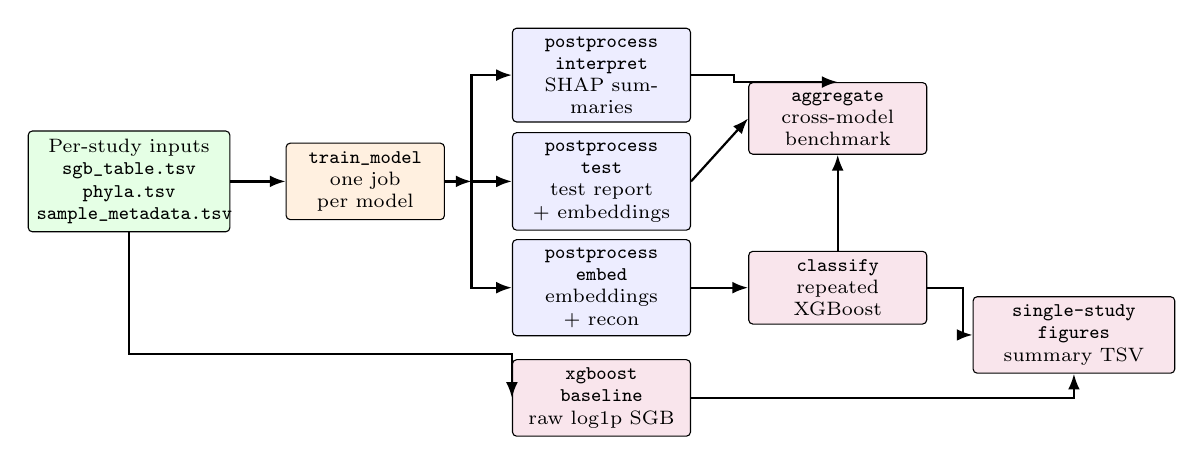
\begin{tikzpicture}[
  x=1cm,y=1cm,
  every node/.append style={font=\scriptsize},
  wide/.style={text width=2.35cm},
  mid/.style={text width=2.05cm},
  narrow/.style={text width=1.8cm}
]
  \node[data, wide] (inp) at (0,0) {Per-study inputs\\\code{sgb_table.tsv}\\\code{phyla.tsv}\\\code{sample_metadata.tsv}};
  \node[model, narrow] (train) at (3.0,0) {\code{train_model}\\one job\\per model};

  \node[block, mid] (interp) at (6.0,1.35) {\ttfamily postprocess\\interpret\\\normalfont SHAP summaries};
  \node[block, mid] (test) at (6.0,0) {\ttfamily postprocess\\test\\\normalfont test report\\+ embeddings};
  \node[block, mid] (embed) at (6.0,-1.35) {\ttfamily postprocess\\embed\\\normalfont embeddings\\+ recon};

  \node[eval, mid] (agg) at (9.0,0.8) {\code{aggregate}\\cross-model\\benchmark};
  \node[eval, mid] (class) at (9.0,-1.35) {\code{classify}\\repeated\\XGBoost};
  \node[eval, mid] (base) at (6.0,-2.75) {\ttfamily xgboost\\baseline\\\normalfont raw log1p SGB};
  \node[eval, wide] (fig) at (12.0,-1.95) {\ttfamily single-study\\figures\\\normalfont summary TSV};

  \coordinate (split) at (4.35,0);
  \draw[arrow] (inp) -- (train);
  \draw[arrow] (train.east) -- (split);
  \draw[arrow] (split) -- (test.west);
  \draw[arrow] (split) |- (interp.west);
  \draw[arrow] (split) |- (embed.west);

  \draw[arrow] (interp.east) -- ++(0.55,0) |- (agg.north);
  \draw[arrow] (test.east) -- (agg.west);
  \draw[arrow] (embed.east) -- (class.west);
  \draw[arrow] (class.east) -- ++(0.45,0) |- (fig.west);

  \draw[arrow] (inp.south) -- ++(0,-1.55) -| (base.west);
  \draw[arrow] (base.east) -- ++(1.25,0) -| (fig.south);
  \draw[arrow] (class.north) -- ++(0,0.55) -| (agg.south);
\end{tikzpicture}}
\vspace{1mm}
\small Entry point: \code{workflow/Snakefile}. In single-study mode, cross-domain DIVA / PhyloDIVA / TAXI models are dropped because a single cohort gives a degenerate domain variable.
\end{frame}

\begin{frame}{Single-study practice}
\small
\textbf{Run}
\begin{center}
\scriptsize
\begin{tabular}{l}
\texttt{snakemake -s workflow/Snakefile \textbackslash}\\
\texttt{  --configfile workflow/config/single\_study.yaml \textbackslash}\\
\texttt{  --cores 8}
\end{tabular}
\end{center}
\textbf{Key config}
\begin{itemize}
  \item \code{data_root}, \code{output_root}, \code{study}, \code{label}.
  \item \code{extra_args}: forwarded to every training CLI, defaulting to Optuna search.
  \item \code{eval_seeds}: default \(\{42,43,44,45,46\}\) for downstream evaluation.
\end{itemize}
\textbf{Interpretation}
\begin{itemize}
  \item Best for within-study reconstruction, embedding quality, and phenotype prediction.
  \item Does not estimate cohort transfer because train and validation folds come from the same study.
  \item Cross-domain wrappers are intentionally excluded.
\end{itemize}
\end{frame}

\begin{frame}{Non-strict LOSO flow}
\centering
\resizebox{0.95\textwidth}{!}{%
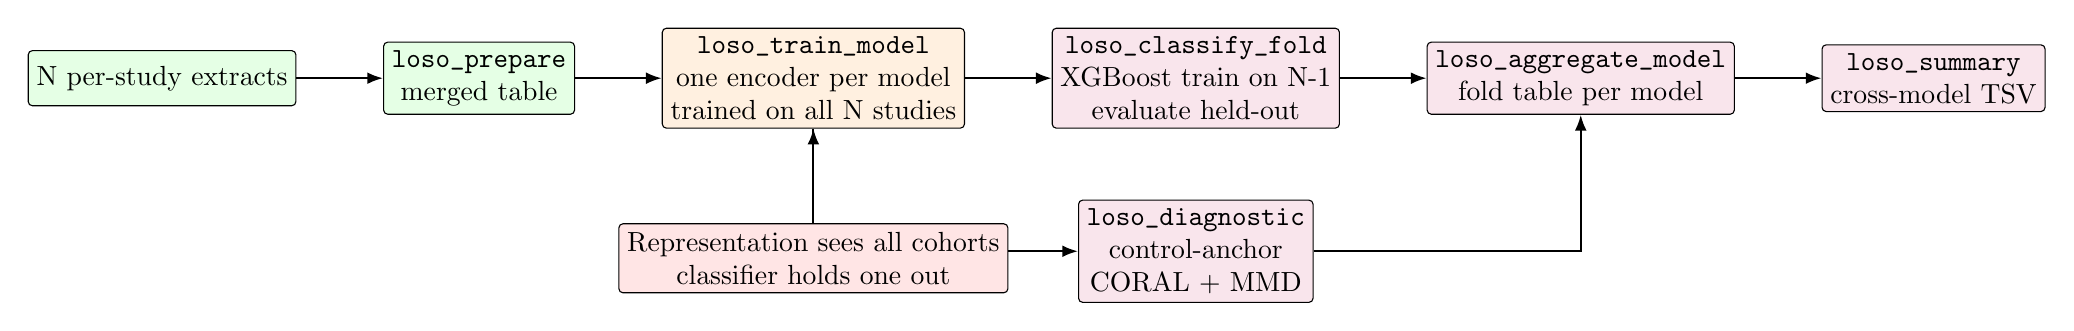
\begin{tikzpicture}[node distance=9mm and 11mm]
  \node[data] (extracts) {N per-study extracts};
  \node[data, right=of extracts] (merge) {\code{loso_prepare}\\merged table};
  \node[model, right=of merge] (train) {\code{loso_train_model}\\one encoder per model\\trained on all N studies};
  \node[eval, right=of train] (folds) {\code{loso_classify_fold}\\XGBoost train on N-1\\evaluate held-out};
  \node[eval, below=of folds] (diag) {\code{loso_diagnostic}\\control-anchor\\CORAL + MMD};
  \node[eval, right=of folds] (agg) {\code{loso_aggregate_model}\\fold table per model};
  \node[eval, right=of agg] (sum) {\code{loso_summary}\\cross-model TSV};
  \draw[arrow] (extracts) -- (merge);
  \draw[arrow] (merge) -- (train);
  \draw[arrow] (train) -- (folds);
  \draw[arrow] (train) |- (diag);
  \draw[arrow] (folds) -- (agg);
  \draw[arrow] (diag) -| (agg);
  \draw[arrow] (agg) -- (sum);
  \node[warn, below=12mm of train] (leak) {Representation sees all cohorts\\classifier holds one out};
  \draw[dashedarrow] (leak) -- (train);
\end{tikzpicture}}
\vspace{1mm}
\small Entry point: \code{workflow/Snakefile.loso}. The encoder is shared across folds, so this is useful but not a fully strict deployment simulation.
\end{frame}

\begin{frame}{Non-strict LOSO practice}
\small
\textbf{Run}
\begin{center}
\scriptsize
\begin{tabular}{l}
\texttt{snakemake -s workflow/Snakefile.loso \textbackslash}\\
\texttt{  --configfile workflow/config/loso\_crc.yaml \textbackslash}\\
\texttt{  --cores 16}
\end{tabular}
\end{center}
\textbf{What it measures}
\begin{itemize}
  \item Downstream classifier transfer: train the classifier on all non-held-out studies and evaluate on the held-out study.
  \item Latent-space study drift: \code{loso_diagnostic} computes control-only CORAL and MMD.
  \item Model comparison under the same XGBoost classifier and five evaluation seeds.
\end{itemize}
\textbf{Caveat}
\begin{itemize}
  \item The encoder and Optuna selection see the held-out cohort because the model is trained once on the merged dataset.
  \item This can be acceptable for exploratory representation analysis, but not for strict external validation.
\end{itemize}
\end{frame}

\begin{frame}{Strict LOSO flow}
\centering
\resizebox{0.98\textwidth}{!}{%
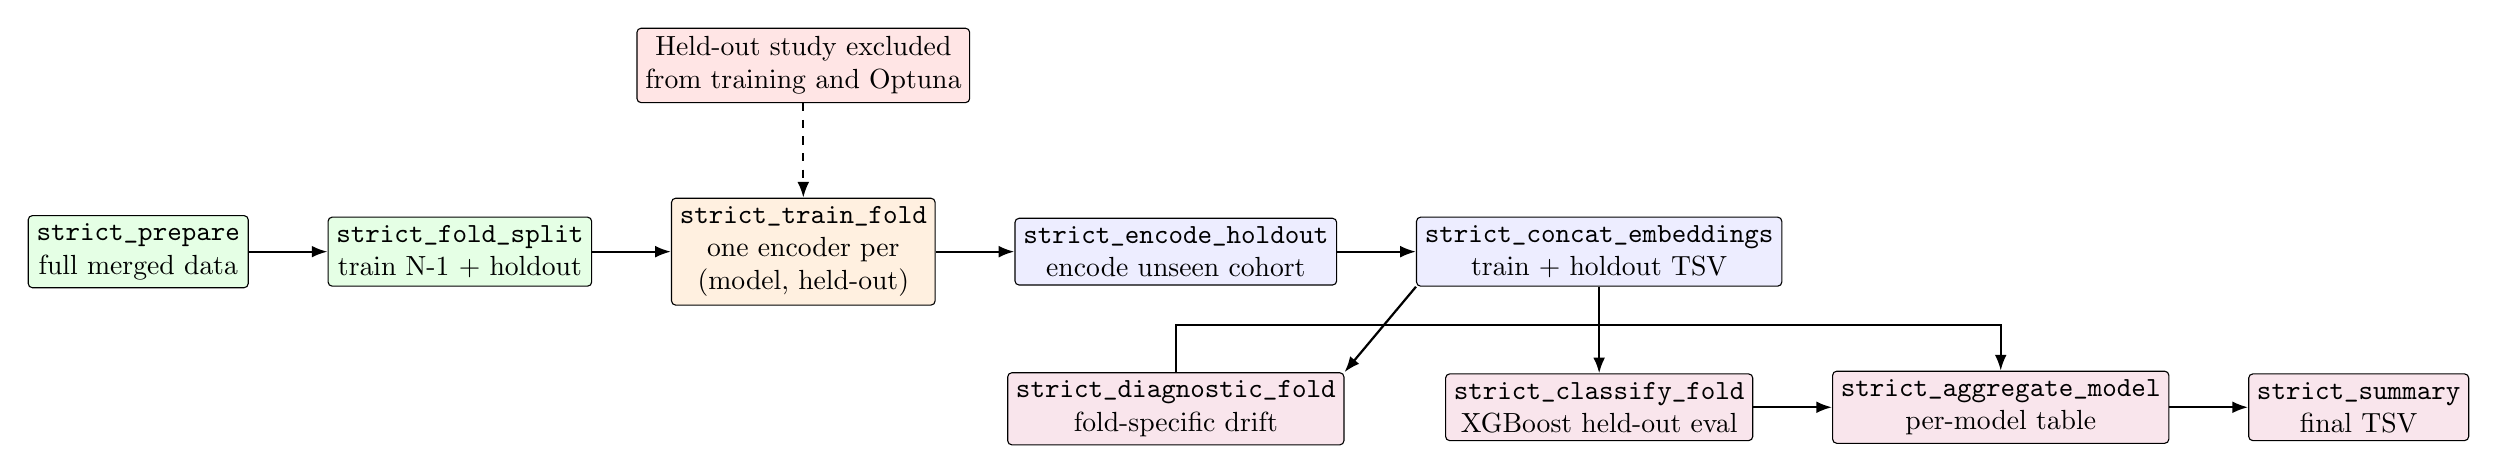
\begin{tikzpicture}[node distance=9mm and 10mm]
  \node[data] (prep) {\code{strict_prepare}\\full merged data};
  \node[data, right=of prep] (split) {\code{strict_fold_split}\\train N-1 + holdout};
  \node[model, right=of split] (train) {\code{strict_train_fold}\\one encoder per\\(model, held-out)};
  \node[block, right=of train] (enc) {\code{strict_encode_holdout}\\encode unseen cohort};
  \node[block, right=of enc] (cat) {\code{strict_concat_embeddings}\\train + holdout TSV};
  \node[eval, below=11mm of cat] (class) {\code{strict_classify_fold}\\XGBoost held-out eval};
  \node[eval, below=11mm of enc] (diag) {\code{strict_diagnostic_fold}\\fold-specific drift};
  \node[eval, right=of class] (agg) {\code{strict_aggregate_model}\\per-model table};
  \node[eval, right=of agg] (sum) {\code{strict_summary}\\final TSV};
  \draw[arrow] (prep) -- (split);
  \draw[arrow] (split) -- (train);
  \draw[arrow] (train) -- (enc);
  \draw[arrow] (enc) -- (cat);
  \draw[arrow] (cat) -- (class);
  \draw[arrow] (cat.south west) -- (diag.north east);
  \draw[arrow] (class) -- (agg);
  \draw[arrow] (diag.north) -- ++(0,6mm) -| (agg.north);
  \draw[arrow] (agg) -- (sum);
  \node[warn, above=12mm of train] (strict) {Held-out study excluded\\from training and Optuna};
  \draw[dashedarrow] (strict) -- (train);
\end{tikzpicture}}
\vspace{1mm}
\small Entry point: \code{workflow/Snakefile.loso_strict}. Cost is about \(N\) times non-strict training.
\end{frame}

\begin{frame}{Strict LOSO practice}
\small
\textbf{Run}
\begin{center}
\scriptsize
\begin{tabular}{l}
\texttt{snakemake -s workflow/Snakefile.loso\_strict \textbackslash}\\
\texttt{  --configfile workflow/config/loso\_strict\_crc.yaml \textbackslash}\\
\texttt{  --cores 16}
\end{tabular}
\end{center}
\textbf{Why it is strict}
\begin{itemize}
  \item For each held-out cohort \(d\), all model fitting uses only \(D \ne d\).
  \item Optuna trials, validation splits, early stopping, and learned encoder weights never see the held-out cohort.
  \item Held-out samples are encoded only after training via \code{biomevae-loso-strict-encode}.
\end{itemize}
\textbf{Cost}
\begin{itemize}
  \item Non-strict: one training run per model.
  \item Strict: \(N\) training runs per model, each usually with its own Optuna search.
\end{itemize}
\end{frame}

\begin{frame}{LOSO model sweep}
\small
\begin{tabular}{p{0.28\textwidth}p{0.36\textwidth}p{0.27\textwidth}}
\toprule
Group & Examples & Default classification slice \\
\midrule
No domain adaptation & \code{hyp-philrvae}, \code{tree-dtm-vae}, \code{beta-vae} & full latent \\
DIVA & \code{diva-tree-dtm-vae}, \code{diva-hyp-philr-nb}, \code{diva-beta-vae} & \(z_y\) \\
PhyloDIVA & \code{phylodiva-tree-dtm-vae}, \code{phylodiva-hyp-philr-nb}, \code{phylodiva-beta-vae} & \(z_y\) \\
TAXI & \code{taxi-tree-dtm-vae}, \code{taxi-hyp-philrvae} & full predictive \(z_\tau \cup z_\rho\) \\
Tree baselines & \code{xgb-baseline}, \code{xgb-coral} & raw or CORAL-aligned SGB features \\
\bottomrule
\end{tabular}
\vspace{2mm}
\begin{itemize}
  \item DIVA / PhyloDIVA use \(z_y\) because it is the class-anchored factor.
  \item TAXI uses the protected plus residual predictive channels, not \(z_d\).
  \item Slice behavior can be overridden in \code{loso_latent_slice}.
\end{itemize}
\end{frame}

\section{PhILR-VAE}

\begin{frame}{PhILR problem setting}
\small
For a sample with \(p\) taxa:
\[
\bm x \in \N_0^p \quad\text{or}\quad \bm x \in \Delta^{p-1},
\qquad
\Delta^{p-1}=\{\bm c\in \R_{>0}^p:\sum_i c_i=1\}.
\]
Counts are closed to a composition with a pseudocount:
\[
c_i=\frac{x_i+\alpha}{\sum_j(x_j+\alpha)}.
\]
\textbf{Modeling goal}
\begin{itemize}
  \item Separate composition from library depth.
  \item Use Euclidean latent-variable machinery in a coordinate system that is correct for compositional data.
  \item Build the coordinate system from the taxonomy tree, not arbitrary feature order.
\end{itemize}
\end{frame}

\begin{frame}{Sequential binary partition balances}
\small
At an internal taxonomy split with descendant leaf groups \(R,S\), cardinalities \(r,s\), define a balance vector \(\bm\psi\in\R^p\):
\[
\psi_i =
\begin{cases}
\sqrt{\dfrac{s}{r(r+s)}} & i\in R,\\[3pt]
-\sqrt{\dfrac{r}{s(r+s)}} & i\in S,\\[3pt]
0 & \text{otherwise}.
\end{cases}
\]
\begin{itemize}
  \item \(\langle \bm\psi,\bm 1\rangle=0\): balances live in the contrast subspace.
  \item \(\|\bm\psi\|_2=1\).
  \item Valid SBP contrasts are mutually orthogonal.
  \item Nodes with \(K>2\) children are linearized into \(K-1\) ordered left-versus-rest splits.
\end{itemize}
Stacking all balances gives
\[
\Psi\in\R^{p\times(p-1)},\qquad \Psi^\top\Psi=I_{p-1},\qquad \operatorname{span}(\Psi)=\bm 1^\perp.
\]
\end{frame}

\begin{frame}{Forward and inverse PhILR}
\small
The Phylogenetic Isometric Log-Ratio transform is
\[
\bm y=\operatorname{ilr}(\bm c)=\log(\bm c)\Psi\in\R^{p-1}.
\]
The inverse used by the decoder is
\[
\widehat{\bm c}=\softmax(\widehat{\bm y}\Psi^\top)\in\Delta^{p-1}.
\]
\textbf{Metric consequence}
\[
\|\bm y^{(1)}-\bm y^{(2)}\|_2
=d_A(\bm c^{(1)},\bm c^{(2)}),
\]
where \(d_A\) is Aitchison distance. Therefore:
\begin{itemize}
  \item A Gaussian in PhILR coordinates is a logistic-normal model on the simplex.
  \item MSE-like reconstruction in PhILR space is geometrically meaningful.
  \item No extra tree-consistency penalty is needed for closure.
\end{itemize}
\end{frame}

\begin{frame}{PhILR-VAE encoder and decoder}
\small
\begin{columns}[T,onlytextwidth]
\column{0.55\textwidth}
\[
p(\bm z)=\mathcal N(\bm0,I_d)
\]
\[
q_\phi(\bm z\mid \bm x)
=\mathcal N\!\left(\bm\mu_\phi(\bm x),
\diag \bm\sigma_\phi^2(\bm x)\right)
\]
\[
\bm x\to\bm c\to\bm y=\log(\bm c)\Psi
\to h_\phi(\bm y)\to(\bm\mu_\phi,\log\bm\sigma_\phi^2)
\]
\[
\bm z=\bm\mu_\phi+\bm\sigma_\phi\odot\bm\varepsilon,\qquad
\bm\varepsilon\sim\mathcal N(\bm0,I)
\]
\column{0.45\textwidth}
\[
\bm z\to g_\theta(\bm z)=\widehat{\bm y}
\]
\[
\widehat{\bm c}=\softmax(\widehat{\bm y}\Psi^\top)
\]
\begin{itemize}
  \item Tree-aware likelihood variants also predict sibling-group concentration parameters.
  \item The same taxonomy backbone and node aggregation are shared with TreeDTM.
\end{itemize}
\end{columns}
\end{frame}

\begin{frame}{PhILR likelihoods}
\small
\begin{tabular}{p{0.27\textwidth}p{0.41\textwidth}p{0.23\textwidth}}
\toprule
Likelihood & Distributional form & Use case \\
\midrule
\code{philr_gaussian} &
\(\bm y\sim \mathcal N(\widehat{\bm y},\diag\bm\sigma_{\rm obs}^2)\) &
relative abundance \\
\code{multinomial} &
\(\bm x\mid N,\widehat{\bm c}\sim\operatorname{Multinomial}(N,\widehat{\bm c})\) &
fixed-depth counts \\
\code{dirichlet_multinomial} &
\(\bm\alpha=\alpha_0\widehat{\bm c}\) then DM marginal &
global overdispersion \\
\code{dirichlet_tree_multinomial} &
product of DM terms over internal sibling groups &
clade-specific count dispersion \\
\code{dirichlet_tree} &
product of continuous Dirichlet densities over sibling fractions &
relative abundance with tree likelihood \\
\bottomrule
\end{tabular}
\end{frame}

\begin{frame}{PhILR Gaussian reconstruction}
\small
For closed relative abundance input:
\[
\bm y=\operatorname{ilr}(\bm c),\qquad
\bm y\mid \bm z \sim
\mathcal N(\widehat{\bm y}_\theta(\bm z),\diag \bm\sigma_{\rm obs}^2).
\]
The negative log-likelihood is
\[
-\log p_\theta(\bm y\mid\bm z)
=\frac12\sum_{k=1}^{p-1}
\left[
\frac{(y_k-\widehat y_k)^2}{\sigma_{{\rm obs},k}^2}
+\log \sigma_{{\rm obs},k}^2
\right]+\text{const}.
\]
\textbf{Interpretation}
\begin{itemize}
  \item This is the logistic-normal likelihood in the original simplex.
  \item The observation scales are learned per PhILR coordinate and clamped for stability.
  \item Library size does not enter because relative input has already been closed.
\end{itemize}
\end{frame}

\begin{frame}{PhILR count likelihoods}
\small
\textbf{Multinomial}
\[
\bm x\mid \widehat{\bm c},N\sim\operatorname{Multinomial}(N,\widehat{\bm c}),
\qquad
-\log p=-\log\binom{N}{\bm x}-\sum_i x_i\log\widehat c_i.
\]
\textbf{Dirichlet-multinomial}
\[
\bm\alpha=\alpha_0\widehat{\bm c},\qquad \alpha_0>0,
\]
\[
-\log p(\bm x\mid\bm\alpha,N)
=-\log\binom{N}{\bm x}
-\log\Gamma(\alpha_0)+\log\Gamma(N+\alpha_0)
-\sum_i\left[\log\Gamma(x_i+\alpha_i)-\log\Gamma(\alpha_i)\right].
\]
\textbf{Tree variants}
\begin{itemize}
  \item PhILR encoder remains unchanged.
  \item Likelihood delegates to the TreeDTM node-aggregated sibling groups.
\end{itemize}
\end{frame}

\begin{frame}{PhILR ELBO}
\small
For any supported likelihood:
\[
\mathcal L_{\rm PhILR}^{(i)}
=-\E_{q_\phi}\log p_\theta(\bm x^{(i)}\mid\bm z)
+\beta_t\,\KL\!\left(q_\phi(\bm z\mid\bm x^{(i)})\,\|\,\mathcal N(\bm0,I)\right)
+\gamma\,\mathcal R(\theta_{\rm lik}).
\]
The Gaussian KL is
\[
\KL
=\frac12\sum_{j=1}^d
\left(\mu_j^2+\sigma_j^2-1-\log\sigma_j^2\right).
\]
\begin{itemize}
  \item \(\beta_t\) is the shared linear KL warm-up schedule.
  \item \(\mathcal R\) regularizes likelihood-specific scales or concentrations.
  \item The objective is likelihood-agnostic except for the NLL term.
\end{itemize}
\end{frame}

\begin{frame}{PhILR computation graph}
\centering
\resizebox{0.93\textwidth}{!}{%
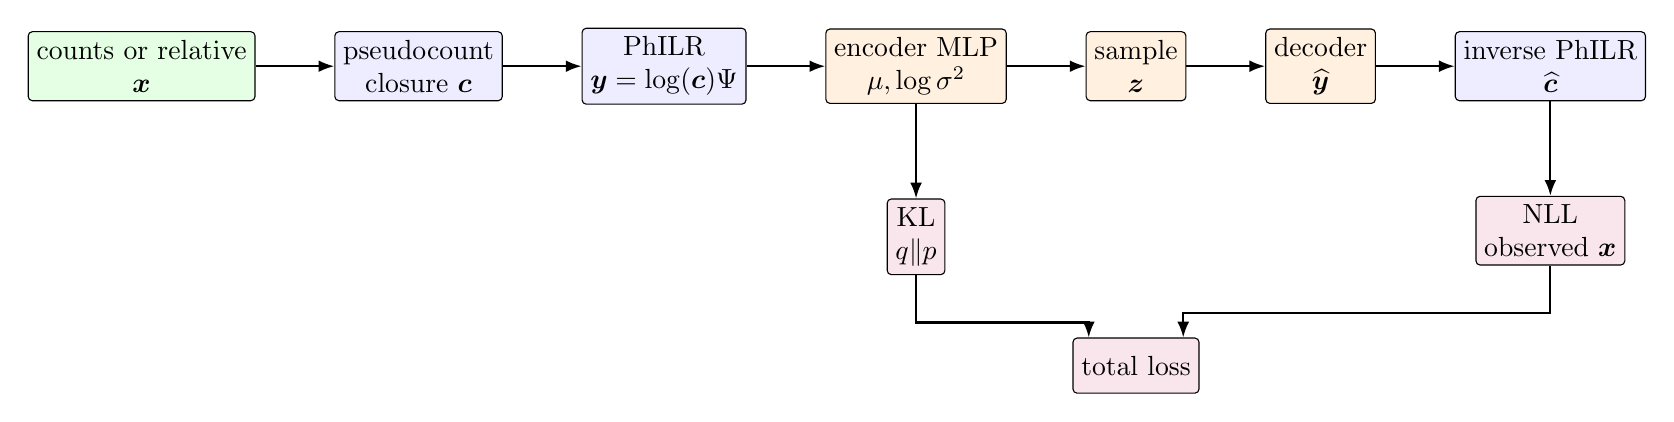
\begin{tikzpicture}[node distance=9mm and 10mm]
  \node[data] (x) {counts or relative\\\(\bm x\)};
  \node[block, right=of x] (close) {pseudocount\\closure \(\bm c\)};
  \node[block, right=of close] (ilr) {PhILR\\\(\bm y=\log(\bm c)\Psi\)};
  \node[model, right=of ilr] (enc) {encoder MLP\\\(\mu,\log\sigma^2\)};
  \node[model, right=of enc] (z) {sample\\\(\bm z\)};
  \node[model, right=of z] (dec) {decoder\\\(\widehat{\bm y}\)};
  \node[block, right=of dec] (inv) {inverse PhILR\\\(\widehat{\bm c}\)};
  \node[eval, below=12mm of enc] (kl) {KL\\\(q\|p\)};
  \node[eval, below=12mm of inv] (nll) {NLL\\observed \(\bm x\)};
  \node[eval, below=30mm of z] (loss) {total loss};
  \draw[arrow] (x) -- (close);
  \draw[arrow] (close) -- (ilr);
  \draw[arrow] (ilr) -- (enc);
  \draw[arrow] (enc) -- (z);
  \draw[arrow] (z) -- (dec);
  \draw[arrow] (dec) -- (inv);
  \draw[arrow] (inv) -- (nll);
  \draw[arrow] (enc) -- (kl);
  \draw[arrow] (kl.south) -- ++(0,-6mm) -| ([xshift=-6mm]loss.north);
  \draw[arrow] (nll.south) -- ++(0,-6mm) -| ([xshift=6mm]loss.north);
\end{tikzpicture}}
\end{frame}

\begin{frame}{Why PhILR is a new core model}
\small
\begin{itemize}
  \item It replaces incoherent independent leaf NB heads for closed compositional data.
  \item It gives exact Aitchison geometry through an orthonormal taxonomy-derived basis.
  \item It keeps library size out of the latent except when the chosen count likelihood reintroduces \(N\) analytically.
  \item It can use five reconstruction likelihoods without changing the encoder geometry.
  \item It shares the same taxonomy graph machinery as TreeDTM, which keeps the training pipeline consistent across new backbones.
\end{itemize}
\end{frame}

\section{TreeDTM-VAE}

\begin{frame}{TreeDTM setup}
\small
Let \(\T\) be a rooted taxonomy tree:
\[
\I=\text{internal nodes},\qquad
\Lleaf=\text{observed leaves},\qquad
K_u=|\Ch(u)|.
\]
For each sample, leaf observations are aggregated to every node:
\[
\bm y\in\R_{\ge 0}^{N},\qquad
y_u=\sum_{v\in\Ch(u)}y_v\quad (u\in\I).
\]
Each internal node \(u\) defines one sibling group
\[
g=(u,\Ch(u)),\qquad K_g=K_u.
\]
\textbf{Core shift from old TreeNB}
\begin{itemize}
  \item Likelihood is placed at internal sibling splits, not independently at leaves.
  \item Dispersion is learned per clade / sibling group.
  \item Closure is enforced locally by multinomial or Dirichlet-family terms.
\end{itemize}
\end{frame}

\begin{frame}{TreeDTM with a tree diagram}
\small
\begin{columns}[T,onlytextwidth]
\column{0.45\textwidth}
\centering
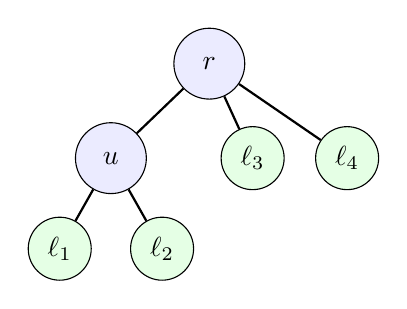
\begin{tikzpicture}[x=1cm,y=1cm]
  \node[treenode] (r) at (0,2.1) {\(r\)};
  \node[treenode] (u) at (-1.25,0.9) {\(u\)};
  \node[treeleaf] (l3) at (0.55,0.9) {\(\ell_3\)};
  \node[treeleaf] (l4) at (1.75,0.9) {\(\ell_4\)};
  \node[treeleaf] (l1) at (-1.9,-0.25) {\(\ell_1\)};
  \node[treeleaf] (l2) at (-0.6,-0.25) {\(\ell_2\)};
  \draw[thick] (r) -- (u);
  \draw[thick] (r) -- (l3);
  \draw[thick] (r) -- (l4);
  \draw[thick] (u) -- (l1);
  \draw[thick] (u) -- (l2);
\end{tikzpicture}
\vspace{1mm}

\scriptsize
\begin{tabular}{ll}
Root group: & \(\Ch(r)=\{u,\ell_3,\ell_4\}\)\\
Clade group: & \(\Ch(u)=\{\ell_1,\ell_2\}\)
\end{tabular}
\column{0.55\textwidth}
\textbf{Observed node counts}
\[
y_u=y_{\ell_1}+y_{\ell_2},\qquad
y_r=y_u+y_{\ell_3}+y_{\ell_4}.
\]
\textbf{Decoder probabilities}
\[
\bm a=h_\theta(\bm z),\qquad
\bm\pi_r=\softmax(a_{r\to u},a_{r\to \ell_3},a_{r\to \ell_4}),
\]
\[
\bm\pi_u=\softmax(a_{u\to \ell_1},a_{u\to \ell_2}).
\]
\textbf{Likelihood factorization}
\[
p(\bm y\mid\bm z)
=p(\bm x_r\mid \bm\pi_r,\alpha_r^0)\,
 p(\bm x_u\mid \bm\pi_u,\alpha_u^0).
\]
Each internal node contributes one local multinomial, Dirichlet-multinomial, or continuous Dirichlet term.
\end{columns}
\end{frame}

\begin{frame}{TreeDTM generative model}
\small
\[
\bm z^{(i)}\sim\mathcal N(\bm0,I_d).
\]
The decoder outputs edge or local split logits:
\[
\bm a^{(i)}=h_\theta(\bm z^{(i)})\in\R^E,
\qquad
E=\sum_{u\in\I}K_u.
\]
For every internal node \(u\), a masked group softmax gives child probabilities:
\[
\pi^{(i)}_{u\to v}
=
\frac{\exp(a^{(i)}_{u\to v})}
{\sum_{v'\in\Ch(u)}\exp(a^{(i)}_{u\to v'})},
\qquad v\in\Ch(u).
\]
\textbf{The same decoder probabilities support three likelihoods}
\begin{itemize}
  \item Tree-multinomial.
  \item Dirichlet-tree-multinomial.
  \item Continuous Dirichlet-tree.
\end{itemize}
\end{frame}

\begin{frame}{Tree-multinomial likelihood}
\small
For internal node \(u\), let child counts be
\[
\bm x_u^{(i)}=(x_v^{(i)})_{v\in\Ch(u)},\qquad
n_u^{(i)}=\sum_{v\in\Ch(u)}x_v^{(i)}.
\]
The local likelihood is
\[
p(\bm x_u^{(i)}\mid \bm\pi_{u,\cdot}^{(i)})
=
\binom{n_u^{(i)}}{\bm x_u^{(i)}}
\prod_{v\in\Ch(u)}
\left(\pi_{u\to v}^{(i)}\right)^{x_{u\to v}^{(i)}}.
\]
The joint log-likelihood is a product over internal nodes:
\[
\log p(\bm y^{(i)}\mid\bm z^{(i)})
=
\sum_{u\in\I}
\log\operatorname{Multinomial}
\left(\bm x_u^{(i)};n_u^{(i)},\bm\pi_{u,\cdot}^{(i)}\right).
\]
\end{frame}

\begin{frame}{Dirichlet-tree-multinomial likelihood}
\small
The default TreeDTM count likelihood adds clade-local overdispersion. For sibling group \(g\):
\[
\bm\alpha_g^{(i)}
=\alpha_g^0\,\bm\pi_g^{(i)}+\epsilon,
\qquad
\alpha_{g,0}^{(i)}=\sum_v\alpha_{g,v}^{(i)}\approx \alpha_g^0.
\]
At internal node \(u\) corresponding to \(g\):
\[
p(\bm x_u^{(i)}\mid \bm\alpha_g^{(i)})
=
\binom{n_u^{(i)}}{\bm x_u^{(i)}}
\frac{\Gamma(\alpha_{g,0}^{(i)})}
{\Gamma(n_u^{(i)}+\alpha_{g,0}^{(i)})}
\prod_{v\in\Ch(u)}
\frac{\Gamma(x_{u\to v}^{(i)}+\alpha_{g,v}^{(i)})}
{\Gamma(\alpha_{g,v}^{(i)})}.
\]
\[
\log p(\bm y^{(i)}\mid\bm z^{(i)})
=\sum_{u\in\I}\log p(\bm x_u^{(i)}\mid \bm\alpha_{g(u)}^{(i)}).
\]
\end{frame}

\begin{frame}{Continuous Dirichlet-tree likelihood}
\small
For relative-abundance data, each internal node contributes a Dirichlet density over observed child fractions:
\[
\bm q_u^{(i)}
=\operatorname{normalise}(\bm x_u^{(i)}+\eta),
\]
\[
\log p(\bm q_u^{(i)}\mid\bm\alpha_g^{(i)})
=
\log\Gamma(\alpha_{g,0}^{(i)})
-\sum_{v\in\Ch(u)}\log\Gamma(\alpha_{g,v}^{(i)})
+\sum_{v\in\Ch(u)}
(\alpha_{g,v}^{(i)}-1)\log q_{u\to v}^{(i)}.
\]
\begin{itemize}
  \item Internal nodes with zero parent mass are masked.
  \item \(\eta\) only keeps fractions inside the Dirichlet support.
  \item This gives a tree-native likelihood without pretending relative abundances are independent leaves.
\end{itemize}
\end{frame}

\begin{frame}{TreeDTM encoder}
\small
The encoder consumes the node-aggregated tensor, then computes sibling-centered log-ratios:
\[
\ell_{u\to v}^{(i)}
=
\log(y_v^{(i)}+\tau)
-
\frac{1}{K_u}\sum_{v'\in\Ch(u)}
\log(y_{v'}^{(i)}+\tau).
\]
\[
\bm\ell^{(i)}=\operatorname{concat}_{u\in\I,v\in\Ch(u)}\ell_{u\to v}^{(i)}.
\]
Then
\[
(\bm\mu_z^{(i)},\log\bm\sigma_z^{2(i)})
=g_\phi(\bm\ell^{(i)}),
\qquad
q_\phi(\bm z\mid\bm y)
=\mathcal N(\bm\mu_z,\diag\bm\sigma_z^2).
\]
\textbf{Why centered?}
\begin{itemize}
  \item Adding the same constant to all children of a node leaves \(\ell\) unchanged.
  \item The encoder feature lives on the same local scale-invariant manifold as the likelihood.
\end{itemize}
\end{frame}

\begin{frame}{TreeDTM training objective}
\small
\[
\mathcal L_{\rm TreeDTM}^{(i)}
=
-\log p_\theta(\bm y^{(i)}\mid\bm z^{(i)})
+\beta_t\KL\!\left(q_\phi(\bm z\mid\bm y^{(i)})\,\|\,\mathcal N(\bm0,I)\right)
+\gamma\mathcal R(\bm\alpha^0).
\]
\[
\KL=
\frac12\sum_j
\left(\mu_{z,j}^2+\sigma_{z,j}^2-1-\log\sigma_{z,j}^2\right).
\]
\begin{itemize}
  \item Free-bits can floor KL per dimension.
  \item \(\mathcal R(\bm\alpha^0)\) is the concentration L2 penalty.
  \item \(\beta_t\) uses the same warm-up resolution as the rest of the package.
\end{itemize}
\end{frame}

\begin{frame}{TreeDTM computation graph}
\centering
\resizebox{0.93\textwidth}{!}{%
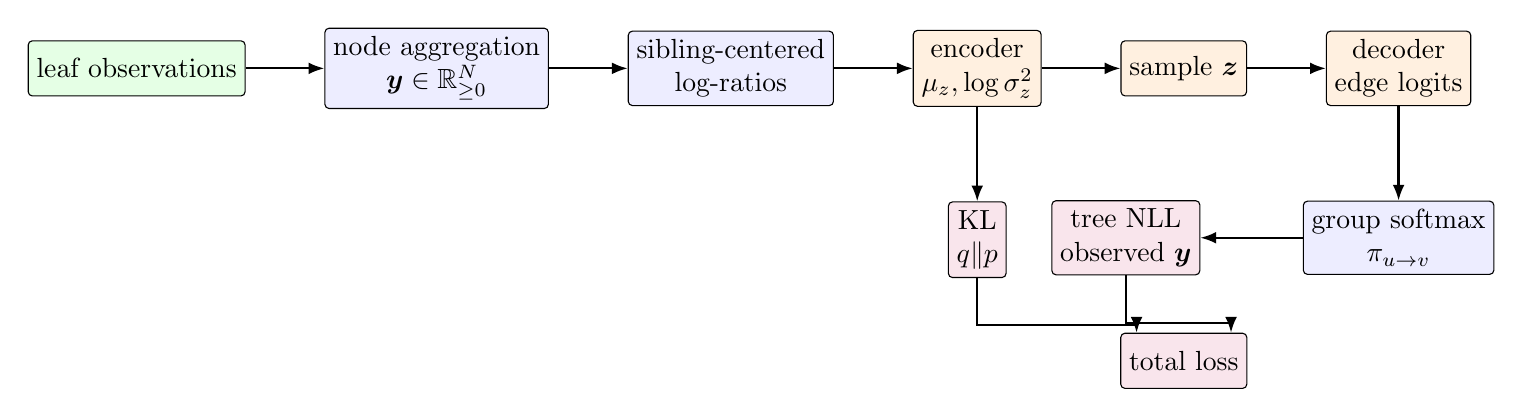
\begin{tikzpicture}[node distance=9mm and 10mm]
  \node[data] (leaf) {leaf observations};
  \node[block, right=of leaf] (agg) {node aggregation\\\(\bm y\in\R^N_{\ge0}\)};
  \node[block, right=of agg] (sclr) {sibling-centered\\log-ratios};
  \node[model, right=of sclr] (enc) {encoder\\\(\mu_z,\log\sigma_z^2\)};
  \node[model, right=of enc] (z) {sample \(\bm z\)};
  \node[model, right=of z] (dec) {decoder\\edge logits};
  \node[block, below=12mm of dec] (sm) {group softmax\\\(\pi_{u\to v}\)};
  \node[eval, left=13mm of sm] (nll) {tree NLL\\observed \(\bm y\)};
  \node[eval, below=12mm of enc] (kl) {KL\\\(q\|p\)};
  \node[eval, below=30mm of z] (loss) {total loss};
  \draw[arrow] (leaf) -- (agg);
  \draw[arrow] (agg) -- (sclr);
  \draw[arrow] (sclr) -- (enc);
  \draw[arrow] (enc) -- (z);
  \draw[arrow] (z) -- (dec);
  \draw[arrow] (dec) -- (sm);
  \draw[arrow] (sm) -- (nll);
  \draw[arrow] (enc) -- (kl);
  \draw[arrow] (kl.south) -- ++(0,-6mm) -| ([xshift=-6mm]loss.north);
  \draw[arrow] (nll.south) -- ++(0,-6mm) -| ([xshift=6mm]loss.north);
\end{tikzpicture}}
\end{frame}

\begin{frame}{Why TreeDTM replaces TreeNB}
\small
\begin{tabular}{p{0.22\textwidth}p{0.35\textwidth}p{0.35\textwidth}}
\toprule
Aspect & Deprecated TreeNB & TreeDTM \\
\midrule
Likelihood location & independent leaves & internal sibling groups \\
Closure & decoder only & likelihood closes each sibling split \\
Dispersion & unrelated leaf parameters & per-clade concentration \(\alpha_g^0\) \\
Encoder & leaf-only log counts & all-node sibling log-ratios \\
Data type & count-like only & counts or relative abundances \\
Statistical target & conflicts with compositional constraints & native tree compositional model \\
\bottomrule
\end{tabular}
\end{frame}

\section{DIVA and PhyloDIVA}

\begin{frame}{DIVA latent partition}
\small
DIVA factorizes the latent:
\[
\bm z=[\bm z_d;\bm z_y;\bm z_x],
\qquad
\bm z_d\in\R^{d_d},\quad
\bm z_y\in\R^{d_y},\quad
\bm z_x\in\R^{d_x}.
\]
Conditional priors:
\[
\begin{aligned}
p(\bm z_d\mid d)&=\mathcal N(\bm\mu_d(d),\diag\bm\sigma_d^2(d)),\\
p(\bm z_y\mid y)&=\mathcal N(\bm\mu_y(y),\diag\bm\sigma_y^2(y)),\\
p(\bm z_x)&=\mathcal N(\bm0,I).
\end{aligned}
\]
Auxiliary classifiers:
\[
q(d\mid\bm z_d)=\softmax\psi_d(\bm z_d),\qquad
q(y\mid\bm z_y)=\softmax\psi_y(\bm z_y).
\]
\end{frame}

\begin{frame}{DIVA objective}
\small
For a labelled sample \((\bm x,d,y)\):
\[
\mathcal L_{\rm DIVA}^{(i)}
=
\underbrace{-\log p_\theta(\bm x^{(i)}\mid\bm z^{(i)})}_{\text{backbone NLL}}
+\beta_t(\KL_d^{(i)}+\KL_y^{(i)}+\KL_x^{(i)})
+\alpha_d\CE_d^{(i)}
+\alpha_y\CE_y^{(i)}.
\]
\[
\KL_d=\KL(q_\phi(\bm z_d\mid\bm x)\,\|\,p(\bm z_d\mid d)),
\quad
\KL_y=\KL(q_\phi(\bm z_y\mid\bm x)\,\|\,p(\bm z_y\mid y)),
\]
\[
\KL_x=\KL(q_\phi(\bm z_x\mid\bm x)\,\|\,\mathcal N(\bm0,I)).
\]
For diagonal Gaussians:
\[
\KL(q\|p)=
\frac12\sum_j\left[
\frac{\sigma_{q,j}^2+(\mu_{q,j}-\mu_{p,j})^2}{\sigma_{p,j}^2}
-1+\log\frac{\sigma_{p,j}^2}{\sigma_{q,j}^2}
\right].
\]
\end{frame}

\begin{frame}{DIVA wrappers in biomevae}
\small
\begin{tabular}{p{0.30\textwidth}p{0.34\textwidth}p{0.28\textwidth}}
\toprule
Wrapper & Backbone likelihood & Main use \\
\midrule
\code{DIVABetaVAE} & Gaussian or MAE-like reconstruction on log-transformed counts & non-taxonomy domain-adaptation control \\
\code{DIVAHyperbolicPhILRVAE} & PhILR compositional likelihoods on Poincare latent geometry & compositional DIVA baseline \\
\code{DIVATreeDTMVAE} & tree-multinomial, Dirichlet-tree-multinomial, Dirichlet-tree & tree-likelihood DIVA baseline \\
\bottomrule
\end{tabular}
\vspace{2mm}
\begin{itemize}
  \item DIVA is likelihood-agnostic: the backbone supplies the NLL.
  \item Downstream LOSO classification normally reads \(z_y\).
  \item Vanilla DIVA encourages \(z_d\) to encode domain, but does not explicitly scrub domain from \(z_y\).
\end{itemize}
\end{frame}

\begin{frame}{PhyloDIVA regularizers}
\small
PhyloDIVA adds three terms to DIVA:
\[
\boxed{
\mathcal L_{\rm PhyloDIVA}
=
\mathcal L_{\rm DIVA}
+\lambda_t\mathcal L_{\rm GRL}
+\mu\mathcal L_{\rm CORAL}
+\nu\mathcal L_{\rm BM}.
}
\]
\textbf{1. Gradient-reversed study critic on \(z_y\)}
\[
\bm z_y \xrightarrow{\operatorname{GRL}(\lambda_t)} \bm z_y'
\xrightarrow{\text{MLP}} \widehat p(d\mid\bm z_y),
\qquad
\mathcal L_{\rm GRL}=-\log\widehat p(d\mid\bm z_y).
\]
\[
\lambda(t)=\lambda_{\max}\left(\frac{2}{1+\exp(-\gamma t)}-1\right).
\]
\textbf{2. Deep CORAL on \(z_x\)}
\[
\mathcal L_{\rm CORAL}
=\frac{1}{|P|}\sum_{(k,k')\in P}\frac{1}{4p^2}
\|\widehat\Sigma_k-\widehat\Sigma_{k'}\|_F^2.
\]
\end{frame}

\begin{frame}{PhyloDIVA tree smoothness}
\small
\textbf{TreeDTM edge smoothness}
\[
\mathcal L_{\rm BM-edge}
=
\frac{1}{|E^\star|}
\sum_{e\in E^\star}
\frac{(a_e-a_{\operatorname{pa}(e)})^2}{\ell_e+\varepsilon}.
\]
\textbf{PhILR coordinate smoothness}
\[
\mathcal L_{\rm BM-coord}
=
\frac{1}{|C^\star|}
\sum_{c\in C^\star}
\frac{(\widehat y_c-\widehat y_{\operatorname{pa}(c)})^2}{\ell_c+\varepsilon}.
\]
\begin{itemize}
  \item With calibrated branch lengths, this is a Brownian-motion prior analogue.
  \item With uncalibrated taxonomies, it is better read as generic tree smoothness.
  \item The smoothness term is the taxonomy-preserving part of PhyloDIVA; the GRL and CORAL terms are the invariance-producing part.
\end{itemize}
\end{frame}

\begin{frame}{DIVA versus PhyloDIVA diagnostics}
\small
\begin{tabular}{p{0.37\textwidth}p{0.25\textwidth}p{0.25\textwidth}}
\toprule
Quantity & DIVA expectation & PhyloDIVA expectation \\
\midrule
Domain accuracy from \(z_d\) & high & high \\
Fresh domain classifier on \(z_y\) & often high leakage & near chance if adversary works \\
Covariance distance of \(z_x\) across studies & nonzero & lower under CORAL \\
Held-out class performance from \(z_y\) & may improve or leak & should improve when study nuisance is separable \\
\bottomrule
\end{tabular}
\vspace{2mm}
\begin{itemize}
  \item These diagnostics are materialized by LOSO summaries and control-anchor reports.
  \item The next section explains why the last row can fail under label shift.
\end{itemize}
\end{frame}

\section{TAXI}

\begin{frame}{TAXI motivation}
\small
TAXI stands for Taxonomy-Anchored eXchangeable Invariance.
\[
z_\tau := \text{protected taxonomy/class latent}\quad(\text{implemented as DIVA }z_y)
\]
\[
z_\rho := \text{residual predictive latent}\quad(\text{implemented as DIVA }z_x)
\]
\[
z_d := \text{study/domain reconstruction latent}.
\]
Instead of marginal invariance,
\[
z_y\perp D,
\]
TAXI enforces conditional residual invariance:
\[
z_\rho \perp D \mid z_\tau,Y.
\]
\textbf{Principle}
\begin{itemize}
  \item Never pass \(z_\tau\) through a GRL.
  \item Use \(z_\tau\) and class context as detached conditioning information.
  \item Scrub only residual study signal from \(z_\rho\).
\end{itemize}
\end{frame}

\begin{frame}{TAXI conditional critic}
\small
The study critic receives
\[
\left[\operatorname{GRL}(z_\rho),\ \operatorname{stopgrad}(z_\tau),\
\operatorname{stopgrad}(y_{\rm ctx})\right].
\]
\[
\mathcal L_{\rm cond\_critic}
=
-\log \widehat p\!\left(d\mid
\operatorname{GRL}(z_\rho),z_\tau,y_{\rm ctx}\right).
\]
The class context is
\[
y_{\rm ctx}=
\begin{cases}
\operatorname{onehot}(y), & \text{labelled sample},\\
\softmax(\text{class logits}), & \text{unlabelled sample}.
\end{cases}
\]
\begin{itemize}
  \item The critic learns to predict study.
  \item The reversed gradient reaches only \(z_\rho\).
  \item The protected taxonomy/class channel \(z_\tau\) remains predictive.
\end{itemize}
\end{frame}

\begin{frame}{TAXI extra losses}
\small
\[
\mathcal L_{\rm TAXI}
=\mathcal L_{\rm DIVA-backbone}
+\lambda_c\mathcal L_{\rm cond\_critic}
+\lambda_{\rm coral}\mathcal L_{\rm cond\_CORAL}
+\lambda_{\rm smooth}\mathcal L_{\rm tree/philr}
+\lambda_{\rm orth}\mathcal L_{\rm orth}
+\lambda_\tau\CE_\tau.
\]
\textbf{Class-conditional CORAL on \(z_\rho\)}
\[
w_i^{(c,d)}=\mathbf 1\{D_i=d\}\,p_i(Y=c),
\qquad
\widehat\Sigma_{c,d}=\operatorname{Cov}_{w^{(c,d)}}(z_\rho),
\]
\[
\mathcal L_{\rm cond\_CORAL}
=
\operatorname{mean}_{c,d<d'}
\frac{\|\widehat\Sigma_{c,d}-\widehat\Sigma_{c,d'}\|_F^2}{4p^2}.
\]
\textbf{Orthogonality}
\[
\mathcal L_{\rm orth}
=
\operatorname{mean}_{c,d}
\|\operatorname{Cov}_{w^{(c,d)}}(z_\tau,z_\rho)\|_F^2.
\]
\end{frame}

\begin{frame}{TAXI wrappers}
\small
\begin{tabular}{p{0.31\textwidth}p{0.34\textwidth}p{0.27\textwidth}}
\toprule
Wrapper & Backbone & Main difference from PhyloDIVA \\
\midrule
\code{TAXIDIVATreeDTMVAE} & DIVA TreeDTM & conditional critic on \(z_\rho\), tree contrast smoothness, class-conditional CORAL \\
\code{TAXIHyperbolicPhILRVAE} & DIVA Hyperbolic PhILR & conditional critic on \(z_\rho\), PhILR coordinate smoothness, class-conditional CORAL \\
\bottomrule
\end{tabular}
\vspace{2mm}
\begin{itemize}
  \item The classifier reads \([z_\tau,z_\rho]\).
  \item \(z_d\) remains the domain reconstruction latent.
  \item CLI aliases accept \code{--latent-tau/--latent-rho} and also \code{--latent-y/--latent-x}.
  \item Default LOSO slice is \code{full} for TAXI so the saved embedding contains the predictive concatenation.
\end{itemize}
\end{frame}

\section{Taxonomy versus Invariance}

\begin{frame}{The conflict}
\small
Two desirable biases can point in opposite directions.
\begin{columns}[T,onlytextwidth]
\column{0.48\textwidth}
\textbf{Taxonomy-aware learning}
\begin{itemize}
  \item Disease signal is smooth on a taxonomy tree.
  \item PhILR and TreeDTM preserve tree-compositional structure.
  \item Smoothness reduces variance and improves finite-sample transfer.
\end{itemize}
\column{0.52\textwidth}
\textbf{Domain invariance}
\begin{itemize}
  \item A held-out study should not be identifiable from the predictive latent.
  \item GRL and CORAL reduce residual study dependence.
  \item If study identity and disease prevalence are linked, invariance can erase predictive taxonomic signal.
\end{itemize}
\end{columns}
\vspace{2mm}
The hard case is label shift:
\[
\mathcal L(Y\mid D=d)\ne \mathcal L(Y\mid D=d').
\]
\end{frame}

\begin{frame}{Formal setup}
\small
Random variables:
\[
X=\text{taxa table},\quad D=\text{study},\quad Y=\text{phenotype},\quad
A(X)=\text{taxonomic state carrying signal}.
\]
For two studies \(d,d'\), define
\[
\Delta_Y=\TV(\mathcal L(Y\mid D=d),\mathcal L(Y\mid D=d')),
\]
\[
\Delta_A=\TV(\mathcal L(A\mid D=d),\mathcal L(A\mid D=d')).
\]
Residual study dependence of an invariant latent:
\[
\delta=
\TV\left(
\mathcal L(Z_{\rm inv}\mid D=d),
\mathcal L(Z_{\rm inv}\mid D=d')
\right).
\]
\begin{itemize}
  \item PhyloDIVA tries to drive \(\delta\) down.
  \item LOSO diagnostics estimate the practical size of taxonomy and latent drift.
\end{itemize}
\end{frame}

\begin{frame}{Taxonomy-aware upper bound}
\small
Assume a tree-smooth target \(f^\star\) with approximation error \(\varepsilon_{\T}^{\rm approx}\):
\[
\Pr\!\left(Y\ne \argmax_c f^\star_{A(X),c}\right)\le
\varepsilon_{\T}^{\rm approx},
\qquad
\Omega_{\T}(f^\star)\le B^2.
\]
For a taxonomy-aware predictor,
\[
\boxed{
R_d(\widehat Y_{\T})
\le
\varepsilon_{\T}^{\rm approx}
+c_1\sqrt{\frac{d_{\T}(\lambda)}{n}}
+c_2\sqrt{\frac{\log(1/\eta)}{n}}
+\lambda B^2
}
\]
where
\[
d_{\T}(\lambda)=
\tr\!\left(L_{\T}(L_{\T}+\lambda I)^{-1}\right).
\]
Informative taxonomy means \(d_{\T}(\lambda)\ll p-1\), so the tree prior reduces variance.
\end{frame}

\begin{frame}{Invariant lower bound}
\small
For any classifier using an invariant latent with
\[
\TV(\mathcal L(Z_{\rm inv}\mid D=d),\mathcal L(Z_{\rm inv}\mid D=d'))\le\delta,
\]
the balanced two-study risk obeys
\[
\boxed{
\frac12\left[
R_d(\widehat Y_{\rm inv})+R_{d'}(\widehat Y_{\rm inv})
\right]
\ge
\frac12(\Delta_Y-\delta)_+.
}
\]
\textbf{Reading}
\begin{itemize}
  \item If the adversary succeeds, \(\delta\to0\).
  \item Under label shift, the lower bound approaches \(\Delta_Y/2\).
  \item Stronger invariance can tighten the lower bound against the model.
\end{itemize}
\end{frame}

\begin{frame}{Crossover condition}
\small
Taxonomy-aware prediction wins when
\[
\frac12(\Delta_Y-\delta)_+
>
\varepsilon_{\T}^{\rm approx}
+c_1\sqrt{\frac{d_{\T}(\lambda)}{n}}
+c_2\sqrt{\frac{\log(1/\eta)}{n}}
+\lambda B^2.
\]
\textbf{Operational meaning}
\begin{itemize}
  \item If \(\Delta_Y\approx\Delta_A\), the disease label shift is carried by taxonomic composition.
  \item A marginal GRL on \(z_y\) cannot distinguish ``study as nuisance'' from ``study as taxonomic disease signal''.
  \item PhILR / TreeDTM without aggressive invariance may outperform PhyloDIVA.
  \item TAXI is designed for this regime: protect \(z_\tau\), align only \(z_\rho\) conditionally.
\end{itemize}
\end{frame}

\begin{frame}{Binary worked example}
\small
Two studies, binary phenotype, binary taxonomic state:
\[
Y=A,\qquad
\Pr(A=1\mid D=0)=0.1,\qquad
\Pr(A=1\mid D=1)=0.9.
\]
Then
\[
\Delta_Y=\Delta_A=0.8.
\]
\textbf{Taxonomy-aware model}
\begin{itemize}
  \item PhILR or TreeDTM can recover the marker clade.
  \item Risk is near \(\varepsilon_{\T}^{\rm approx}\), up to finite-sample error.
\end{itemize}
\textbf{Strict marginal invariance}
\begin{itemize}
  \item If \(\delta=0\), the invariant lower bound is at least \(0.4\).
  \item In the symmetric example, any domain-independent output has balanced risk \(0.5\).
\end{itemize}
\end{frame}

\begin{frame}{Practical knob interpretation}
\small
\begin{tabular}{p{0.23\textwidth}p{0.30\textwidth}p{0.30\textwidth}}
\toprule
Knob & Helps taxonomy bound & Affects invariance bound \\
\midrule
\code{--smooth-weight} & lowers effective tree complexity when tuned well & no direct effect on \(\delta\) \\
\code{--grl-lambda} & no direct effect & reduces \(\delta\), which can hurt under label shift \\
\code{--coral-weight} & no direct effect & reduces second-order study drift \\
\code{--alpha-y} & sharpens \(z_y\) as class latent & may increase study dependence if labels are study-shifted \\
TAXI \code{--lambda-cond-*} & preserves \(z_\tau\) signal & aligns only residual \(z_\rho\) conditionally \\
\bottomrule
\end{tabular}
\vspace{2mm}
\begin{itemize}
  \item Use control-anchor diagnostics to decide whether study drift is nuisance or taxonomic signal.
  \item Compare strict and non-strict LOSO to quantify representation-side leakage.
\end{itemize}
\end{frame}

\section{Operational Summary}

\begin{frame}{Choosing a pipeline}
\small
\begin{tabular}{p{0.25\textwidth}p{0.37\textwidth}p{0.29\textwidth}}
\toprule
Goal & Use & Caveat \\
\midrule
Within-study benchmarking & Single-study \code{workflow/Snakefile} & no external cohort transfer \\
Fast cross-cohort screening & Non-strict \code{Snakefile.loso} & encoder sees all cohorts \\
Deployment-like external validation & Strict \code{Snakefile.loso_strict} & \(N\)-times more model training \\
Diagnose study drift & LOSO diagnostics & compare within class, especially controls \\
Attribute domain adaptation gains & compare beta, DIVA-beta, XGB, XGB-CORAL rows & same labels and seeds required \\
\bottomrule
\end{tabular}
\end{frame}

\begin{frame}{Choosing a model}
\small
\begin{itemize}
  \item Start with \code{tree-dtm-vae} and \code{philrvae}/\code{hyp-philrvae} when the data are compositional and taxonomy is reliable.
  \item Use DIVA when domain effects are strong and plausibly separable from phenotype signal.
  \item Use PhyloDIVA when you want DIVA plus explicit latent study scrubbing, CORAL residual alignment, and tree smoothness.
  \item Use TAXI when the phenotype signal is likely taxonomic and study-shifted, so marginal \(z_y\) invariance may over-scrub.
  \item Always compare against \code{xgb-baseline}; a VAE row that does not beat raw-feature XGBoost is not earning its complexity.
\end{itemize}
\end{frame}

\begin{frame}{Artifacts to inspect}
\small
\begin{tabular}{p{0.32\textwidth}p{0.52\textwidth}}
\toprule
Artifact & What to read \\
\midrule
\code{training_log.tsv} & convergence, KL warm-up, auxiliary and adaptation losses \\
\code{config.json} & selected hyperparameters, latent dimensions, likelihood \\
\code{embeddings*.tsv} & full latent and DIVA/TAXI slices \\
\code{classification_results.json} & per-seed XGBoost metrics and fold sizes \\
\code{loso_summary.tsv} & cross-model held-out performance table \\
\code{control_anchor_summary.json} & control-only MMD and CORAL drift diagnostics \\
\code{optuna_best_params.json} & best trial configuration after HPO \\
\bottomrule
\end{tabular}
\end{frame}

\begin{frame}{Implementation map}
\small
\begin{tabular}{p{0.35\textwidth}p{0.45\textwidth}}
\toprule
Concept & Code \\
\midrule
PhILR basis and transform & \code{src/biomevae/models/philrvae.py}, \code{taxonomy_tree.py} \\
TreeDTM likelihood and topology & \code{src/biomevae/models/tree_dtm_vae.py} \\
DIVA core & \code{src/biomevae/models/diva.py} \\
PhyloDIVA adaptation losses & \code{src/biomevae/models/phylo_da.py}, \code{phylo_cov.py} \\
TAXI conditional invariance & \code{src/biomevae/models/taxi_treedtmvae.py}, \code{taxi_hyp_philrvae.py} \\
LOSO preparation and classification & \code{src/biomevae/loso.py}, \code{src/biomevae/cli/loso_classify.py} \\
Snakemake rules & \code{workflow/rules/*.smk} \\
\bottomrule
\end{tabular}
\end{frame}

\begin{frame}{Takeaways}
\small
\begin{itemize}
  \item PhILR-VAE is the Aitchison-correct compositional backbone: taxonomy defines an orthonormal ILR basis, and likelihoods respect either the simplex or fixed-depth count table.
  \item TreeDTM-VAE is the tree-native count/relative likelihood backbone: reconstruction happens through local sibling distributions and clade-level overdispersion.
  \item DIVA partitions representation by domain, label, and residual factors; PhyloDIVA strengthens invariance and smoothness.
  \item TAXI protects the taxonomy/class channel and aligns only the residual predictive channel conditionally.
  \item Strict LOSO is the decisive external-validation pipeline; non-strict LOSO is useful for screening but has representation-side leakage.
  \item Under label shift, taxonomy regularization and domain invariance can be mathematically opposed. Diagnostics should guide which bias to trust.
\end{itemize}
\end{frame}

\begin{frame}{References in the repository}
\small
\begin{itemize}
  \item \code{docs/philrvae_theory.md}
  \item \code{docs/tree_dtm_vae_theory.md}
  \item \code{docs/diva_theory.md}
  \item \code{docs/phylodiva_theory.md}
  \item \code{docs/taxonomy_vs_domain_invariance_theorem.md}
  \item \code{workflow/README.md} and \code{workflow/README_loso.md}
  \item \code{workflow/Snakefile}, \code{workflow/Snakefile.loso}, \code{workflow/Snakefile.loso_strict}
\end{itemize}
\vspace{2mm}
\small External methods named in the docs: DIVA (Ilse et al. 2020), DANN/GRL (Ganin and Lempitsky 2015), Deep CORAL (Sun and Saenko 2016), Brownian-motion tree priors (Felsenstein 1985), and domain-adaptation lower bounds.
\end{frame}

\end{document}
